\section{Reservoir ComputingとしてのRecurrent SNNの教師あり学習}
この章ではReservoir ComputingとしてのRecurrent SNNと、それを学習するためのFORCE法について解説します。
\section{Reservoir Computing}
\textbf{Reservoir Computing}\index{Reservoir Computing}は、RNN\footnote{ここでは発火率モデルについてのRNNについて述べています。}のモデルの一種です。一般のRNNが全ての結合重みを学習するのに対し、Reservoir ComputingではRNNのユニット間の結合重みはランダムに初期化して固定し、\textbf{出力の結合重みだけを学習}\index{しゅつりょくのけつごうおもみだけをがくしゅう@出力の結合重みだけを学習}します。そのため、Reservoir Computingは学習するパラメータが少なく、学習も高速に行えます(もちろん関数の表現力は一般のRNNの方が優れています)。\par
Reservoirというのは溜め池(貯水池)を意味します。Reservoir Computingでは、まず入力信号をランダムな固定重みにより高次空間の信号に変換し、Reservoir RNN(信号の溜め池)に保持します。そして、Reservoir RNNのユニットの活動として保持された情報を学習可能な重みにより線形変換し、出力とします。このとき、ネットワークの出力が教師信号と一致するように出力重みを更新します。
%\begin{comment}
\begin{figure}[htbp]
    \centering
    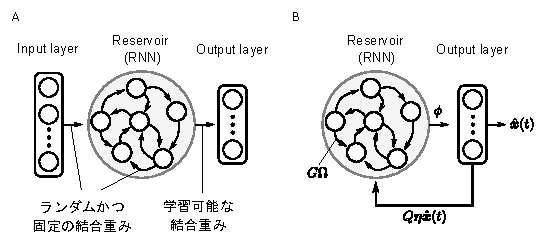
\includegraphics[scale=1.2]{figs/reservoir_computing.pdf}
    \caption{(A)Reservoir Computingの一般的なモデル。入力と中間にはランダムに固定された重みを用い、出力のみ学習可能となっています。 (B)FORCE法で用いるモデルの1つ。7.3節以降でこのモデルの実装を行います。}
    \label{fig:RC}
\end{figure}
%\end{comment}
\subsection{FORCE法とRecurrent SNNへの適用}
Reservoir Computingにおける教師あり学習の手法の1つとして、\textbf{FORCE法}と呼ばれるものがあります。\textbf{FORCE} (First-Order Reduced and Controlled Error)法は(Sussillo \& Abbott, 2009)で提案された学習法で、元々は発火率ベースのRNNに対するオンラインの学習法です (具体的な方法については次節で解説します)。さらに(Nicola \& Clopath, 2017)はFORCE法がRecurrent SNNの学習に直接的に使用できる、ということを示しました。この章では(Nicola \& Clopath, 2017)の手法を用いてReservoir ComputingとしてのRecurrent SNNの教師あり学習を行います。
\subsubsection{Recurrent SNNに正弦波を学習させる}
今回はRecurrent SNNのニューロンの活動をデコードしたものが正弦波となるように(すなわち正弦波を教師信号として)訓練することを目標とします。先になりますが、結果は図のようになります。
\subsubsection{ネットワークの構造と教師信号}
ネットワークの構造は図のようになっています。ネットワークには特別な入力があるわけではなく、再帰的な入力によって活動が持続しています(膜電位の初期値をランダムにしているため開始時に発火するニューロン\footnote{ここでの「ニューロン」はこれ以後も含め、Reservoirのユニットを指します。}があり、またバイアス電流もあります)。\par
まず、Reservoirニューロンの数を$N$とし、出力の数を$N_\text{out}$とします。$i$番目のニューロンの入力はバイアス電流を$I_{\text{Bias}}$として、
\begin{equation}
I_i=s_i+I_{\text{Bias}}    
\end{equation}
と表されます。ただし、$s_i$は 
\begin{equation}
s_{i}=\sum_{j=1}^{N} \omega_{i j} r_{j}    
\end{equation}
として計算されます。$r_j$が$j$番目のニューロンの出力(シナプスフィルターをかけられたスパイク列), $\omega_{i j}$は$j$番目のニューロンから$i$番目のニューロンへの結合重みを意味します。\par
次にニューロンの活動$r_j$を重み$\phi\in \mathbb{R}^{N\times N_\text{out}}$で線形にデコードし、その出力$\hat{\boldsymbol{x}}(t)$を教師信号$\boldsymbol{x}(t)$に近づけます。すなわち、
\begin{equation}
\hat{\boldsymbol{x}}(t)=\sum_{j=1}^{N} \boldsymbol{\phi}_j r_{j}=\phi^\intercal\boldsymbol{r}
\end{equation}
とします。ただし、$^\intercal$を転置記号とし、$\boldsymbol{x}$を列ベクトル、$\boldsymbol{x}^\intercal$を行ベクトルとします。また、$\boldsymbol{\phi}_j\in \mathbb{R}^{N_\text{out}}$です。\par
ここから少しややこしいのですが、ネットワークの重み$\Omega=[\omega_{ij}]\in \mathbb{R}^{N\times N}$は 
\begin{equation}
\omega_{i j}=G \omega_{i j}^{0}+Q \boldsymbol{\eta}_{i}^\intercal \boldsymbol{\phi}_j 
\end{equation}
となっています。$\omega_{i j}^{0}$は固定された再帰重みです。$G, Q$は定数で、$\eta=[\boldsymbol{\eta}_{i}^\intercal]\in \mathbb{R}^{N\times N_\text{out}}$は$-1$か1に等確率に決められた行列です。よって学習するパラメータは$\phi$のみです。よってバイアスを抜いた入力電流$s_{i}$は次のように分割できます。
\begin{align}
s_{i}&=\sum_{j=1}^{N} \omega_{i j} r_{j}\\
&=\sum_{j=1}^{N} \left(G \omega_{i j}^{0}+Q \boldsymbol{\eta}_{i}^\intercal \boldsymbol{\phi}_j \right)r_{j}\\
&=Q\boldsymbol{\eta}_{i}^\intercal \hat{\boldsymbol{x}}(t)+\sum_{j=1}^{N} G \omega_{i j}^{0}r_{j}
\end{align}
\subsubsection{固定重みの初期化}
固定された結合重み$\omega_{i j}^{0}$は$\mathcal{N}(0, (Np)^{-1})$の正規分布からランダムサンプリングした値です($N$はニューロンの数、$p$は定数)。ただし、各ニューロンが投射される重みの平均が0になるようにスケーリングします。
\subsection{RLS法による重みの更新}
\footnote{ModelDBにおいて公開されているMATLABのコード(\url{https://senselab.med.yale.edu/ModelDB/ShowModel.cshtml?model=190565})を参考にしました。}
FORCE法は\textbf{RLSフィルタ}(recursive least squares filter, 再帰的最小二乗法フィルタ)という\textbf{適応フィルタ}(adaptive filter)の一種を学習するアルゴリズムを、RNNの学習に適応したものです\footnote{なお、(Sussillo \& Abbott, 2009)ではDelta則を用いることで、RLS法を用いない重みの更新則も紹介されています。}。
誤差を 
\begin{equation}
\boldsymbol{e}(t)=\hat{\boldsymbol{x}}(t)-\boldsymbol{x}(t)=\phi(t-\Delta t)^\intercal \boldsymbol{r}(t)-\boldsymbol{x}(t)    
\end{equation}
とした場合\footnote{実際にはこれは真の誤差ではなく、事前誤差(apriori error)と呼ばれるものです。真の誤差は$\phi(t)^\intercal \boldsymbol{r}(t)-\boldsymbol{x}(t)$と表されます。}、出力重み$\phi$を次の式で更新します。
\begin{align}
\phi(t)&=\phi(t-\Delta t)-P(t) \boldsymbol{r}(t)\boldsymbol{e}(t)^\intercal\\
P(t)&=P(t-\Delta t)-\frac{P(t-\Delta t) \boldsymbol{r}(t) \boldsymbol{r}(t)^\intercal P(t-\Delta t)}{1+\boldsymbol{r}(t)^\intercal P(t-\Delta
t) \boldsymbol{r}(t)} 
\end{align}
また、初期値は$\phi(0)=0,
P(0)=I_{N}\lambda^{-1}$です。$I_{N}$は$N$次の単位行列を意味します。$\lambda$は正則化のための定数です。
\subsubsection{FORCE法の実装}
それではFORCE法の実装をしてみましょう\footnote{コードは\texttt{./TrainingSNN/LIF\_FORCE\_sinewave.py}です。}。Reservoirネットワークは2000個のLIFニューロンで構成されているとします。また出力ユニットの個数は1です。まず、各種定数と教師信号を定義します。
\begin{lstlisting}[language=julia]
N = 2000  # ニューロンの数
dt = 5e-5 # タイムステップ(s)
tref = 2e-3 # 不応期(s)
tc_m = 1e-2 # 膜時定数(s)
vreset = -65 # リセット電位(mV) 
vrest = 0 # 静止膜電位(mV)
vthr = -40 # 閾値電位(mV)
vpeak = 30 # ピーク電位(mV)
BIAS = -40 # 入力電流のバイアス(pA)
td = 2e-2; tr = 2e-3 # シナプスの時定数(s)
alpha = dt*0.1  
P = np.eye(N)*alpha
Q = 10; G = 0.04

T = 15 # シミュレーション時間 (s)
tmin = round(5/dt) # 重み更新の開始ステップ
tcrit = round(10/dt) # 重み更新の終了ステップ
step = 50 # 重み更新のステップ間隔
nt = round(T/dt) # シミュレーションステップ数
zx = np.sin(2*np.pi*np.arange(nt)*dt*5) # 教師信号
\end{lstlisting}
次にニューロンとシナプスを定義します。
\begin{lstlisting}[language=julia]
from Models.Neurons import CurrentBasedLIF
from Models.Synapses import DoubleExponentialSynapse

# ニューロンとシナプスの定義 
neurons = CurrentBasedLIF(N=N, dt=dt, tref=tref, tc_m=tc_m,
                          vrest=vrest, vreset=vreset, vthr=vthr, vpeak=vpeak)
neurons.v = vreset + np.random.rand(N)*(vpeak-vreset) # 膜電位の初期化

synapses_out = DoubleExponentialSynapse(N, dt=dt, td=td, tr=tr)
synapses_rec = DoubleExponentialSynapse(N, dt=dt, td=td, tr=tr)

# 再帰重みの初期値
p = 0.1 # ネットワークのスパース性
OMEGA = G*(np.random.randn(N,N))*(np.random.rand(N,N)<p)/(np.sqrt(N)*p)
for i in range(N):
    QS = np.where(np.abs(OMEGA[i,:])>0)[0]
    OMEGA[i,QS] = OMEGA[i,QS] - np.sum(OMEGA[i,QS], axis=0)/len(QS)
\end{lstlisting}
シナプスのインスタンスとして\texttt{synapses\_out, synapses\_rec}があります。実は\texttt{synapses\_out}だけでも良いのですが、高速化のために2つ用意しています。また、\texttt{OMEGA}はランダムに生成した後にスケーリングをしています。次に各種変数の初期化と、記録用変数を定義します。
\begin{lstlisting}[language=julia]
# 変数の初期値
k = 1 # 出力ニューロンの数
E = (2*np.random.rand(N, k) - 1)*Q
PSC = np.zeros(N).astype(np.float32) # シナプス後電流
JD = np.zeros(N).astype(np.float32) # 再帰入力の重み和
z = np.zeros(k).astype(np.float32) # 出力の初期化
Phi = np.zeros(N).astype(np.float32) # 学習される重みの初期値

# 記録用変数 
REC_v = np.zeros((nt,10)).astype(np.float32) # 膜電位の記録変数
current = np.zeros(nt).astype(np.float32) # 出力の電流の記録変数
tspike = np.zeros((4*nt,2)).astype(np.float32) # スパイク時刻の記録変数
ns = 0 # スパイク数の記録変数 
\end{lstlisting}
それではシミュレーションのメインの部分を書いていきましょう。
\begin{lstlisting}[language=julia]
for t in tqdm(range(nt)):
    I = PSC + np.dot(E, z) + BIAS # シナプス電流 
    s = neurons(I) # 中間ニューロンのスパイク
    
    index = np.where(s)[0] # 発火したニューロンのindex
    len_idx = len(index) # 発火したニューロンの数
    if len_idx > 0:
        JD = np.sum(OMEGA[:, index], axis=1)  
        tspike[ns:ns+len_idx,:] = np.vstack((index, 0*index+dt*t)).T
        ns = ns + len_idx # スパイク数の記録

    PSC = synapses_rec(JD*(len_idx>0)) # 再帰的入力電流
    #PSC = np.dot(OMEGA, r) # 遅い
    r = synapses_out(s) # 出力電流(神経伝達物質の放出量)  
    r = np.expand_dims(r,1) # (N,) -> (N, 1)
    z = np.dot(Phi.T, r) # デコードされた出力
    err = z - zx[t] # 誤差

    # FORCE法(RLS)による重み更新
    if t % step == 1:
        if t > tmin:
            if t < tcrit:
                cd = np.dot(P, r)
                Phi = Phi - np.dot(cd, err.T)
                P = P - np.dot(cd, cd.T) / (1.0 + np.dot(r.T, cd)
    
    current[t] = z # デコード結果の記録
    REC_v[t] = neurons.v_[:10] # 膜電位の記録
\end{lstlisting}
途中で少し不思議に思われるようなことをしています。\\
\colorbox{shadecolor}{\texttt{PSC = synapses\_rec(JD*(len\_idx>0))}}の部分(とその少し上)ですが、これはデコードに用いる\texttt{r}を行列変換するよりも発火した結合重みの和を取り、再帰入力のシナプス後細胞のモデルに入力した方が速いという理由によります。\texttt{t}が一定のステップの範囲にある場合はFORCE法により学習を実行します。最後に各種変数を記録しています。\par
それでは学習後の結果を表示しましょう。初めに発火数と発火率を表示し、次に学習前と学習後の5つのニューロンの膜電位、最後に学習前/中間と学習後のデコード結果を描画します(なお、この本に記載はしていないですがコードには重みの固有値の描画も付けています)。
\begin{lstlisting}[language=julia]
TotNumSpikes = ns 
M = tspike[tspike[:,1]>dt*tcrit,:]
AverageRate = len(M)/(N*(T-dt*tcrit))
print("\n")
print("Total number of spikes : ", TotNumSpikes)
print("Average firing rate(Hz): ", AverageRate)
step_range = 20000
plt.figure(figsize=(10, 5))
plt.subplot(1,2,1)
for j in range(5):
    plt.plot(np.arange(step_range)*dt,
             REC_v[:step_range, j]/(50-vreset)+j, color="k")
plt.title('Pre-Learning')
plt.xlabel('Time (s)'); plt.ylabel('Neuron Index') 
plt.subplot(1,2,2)
for j in range(5):
    plt.plot(np.arange(nt-step_range, nt)*dt,
             REC_v[nt-step_range:, j]/(50-vreset)+j,
             color="k")
plt.title('Post Learning'); plt.xlabel('Time (s)')
plt.show()

plt.figure(figsize=(10,5))
plt.subplot(1,2,1)
plt.plot(np.arange(nt)*dt, zx, label="Target", color="k")
plt.plot(np.arange(nt)*dt, current, label="Decoded output",
         linestyle="dashed", color="k")
plt.xlim(4.5,5.5); plt.ylim(-1.1,1.4)
plt.title('Pre/peri Learning')
plt.xlabel('Time (s)'); plt.ylabel('current') 
plt.subplot(1,2,2)
plt.title('Post Learning')
plt.plot(np.arange(nt)*dt, zx, label="Target", color="k")
plt.plot(np.arange(nt)*dt, current, label="Decoded output",
         linestyle="dashed", color="k")
plt.xlim(14,15); plt.ylim(-1.1,1.4)
plt.xlabel('Time (s)'); plt.legend(loc='upper right')
plt.show()
\end{lstlisting}
結果は図\ref{fig:LIF_FORCE_1}, \ref{fig:LIF_FORCE_2}のようになります。また、同様のシミュレーションをIzhikevichニューロンで行った\footnote{コードは\texttt{./TrainingSNN/Izhikevich\_FORCE\_sinewave.py}です。}結果も示しています。
\begin{figure}[htbp]
    \centering
    \includegraphics[scale=0.4]{figs/LIF_FORCE_prepost.pdf}
    \includegraphics[scale=0.4]{figs/Iz_FORCE_prepost.pdf}
    \caption{FORCE法による学習前(左)と学習後(右)の発火率の変化。(上)LIFニューロン、(下)をIzhikevichニューロン}
    \label{fig:LIF_FORCE_1}
\end{figure}
\begin{figure}[H]
    \centering
    \includegraphics[scale=0.4]{figs/LIF_FORCE_decoded.pdf}
    \caption{FORCE法による学習前(左)と学習後(右)のデコード結果の変化(LIFニューロンの場合)。教師信号は実線、デコード結果は破線で示している。}
    \label{fig:LIF_FORCE_2}
\end{figure}
\subsection{鳥の鳴き声の再現と海馬の記憶と再生}
(Nicola \& Clopath, 2017)では教師信号として正弦波以外にもVan der Pol方程式やLorenz方程式の軌道を用いて実験しています。さらに教師信号としてベートーヴェンの歓喜の歌(Ode to joy)や鳥の鳴き声を用いても学習可能であったようです。\par
話は少しずれますが、小鳥の運動前野である\textbf{HVC}には連鎖的に結合したニューロン群が存在します。これはリズムを生み出すための計時に関わっているといわれています。カナリアのHVCニューロンを実験的に損傷(ablation)させると歌が歌えなくなるという実験がありますが、同様にSNNのHVCパターンをablationすると学習した歌が再生できなくなったようです。このような計時に関わるパターンを\textbf{HDTS}(high-dimentional temporal signal)とNicolaらは呼んでいます。HDTSを学習させた後に歓喜の歌を学習させると、HDTSがない場合よりも短い時間かつ高精度で学習できたようです。\par
さらにHDTSを外部入力とし、同時に映像を学習させる、という実験もしています(HDTSを内的に学習させる場合も行っています)。ネットワークは記録した映像を実時間で再生することができましたが、外部信号のHDTSを加速させることで圧縮再生が可能だったそうです。さらにHDTSを逆にすると、逆再生もできたそうです。\par
ニューロンの発火のタスク依存的な圧縮は実験的に観察されています(例えばEuston, et al., 2007)。空間的な課題(箱の中に入れて探索させるなど)をラットにさせると、課題中に記憶された場所細胞の順序だった活動は、ラットの睡眠中に圧縮再生されるという実験結果があります。その圧縮比は5.4〜8.1だったそうですが、この比率はSNNが映像を大きな損失なく再生できる圧縮比とほぼ同じであったようです。Nicolaらはさらに進んでSNNを用いて海馬における急速圧縮学習の機構における介在細胞の働きについての研究も行っています(Nicola \& Clopath, 2019)。
\section{RLS法の導出}
ここからはRLS法の導出を行います(cf. Haykin, 2002)。RLS法では次の損失関数$C\in \mathbb{R}^{N_\text{out}}$を最小化するような重み$\phi=[\boldsymbol{\phi}_j]\in \mathbb{R}^{N\times N_\text{out}}$を求めます。シミュレーション時間を$T$とすると、$C$は
\begin{equation}
C=\int_{0}^T(\hat{\boldsymbol{x}}(t)-\boldsymbol{x}(t))^{2} \mathrm{d} t+\lambda \phi^\intercal \phi
\end{equation}
です。ただし、$\hat{\boldsymbol{x}}(t), \boldsymbol{x}(t) \in \mathbb{R}^{N_\text{out}}$です。\par
さて、式の$C$を最小化するような$\phi$を数値的に求めるためには、損失関数の近似が必要です。まず、
時間幅$\Delta t$で$C$を離散化します。さらに$n$ステップ目における重み$\phi(n)$により、$\hat{\boldsymbol{x}}(i)\simeq \phi(n)^\intercal \boldsymbol{r}(i)$と近似します。このとき、$n$ステップ目の損失関数$C(n)$は
\begin{align}
C(n)&\simeq \sum_{i=0}^{n}(\hat{\boldsymbol{x}}(i)-\boldsymbol{x}(i))^{2}+\lambda \phi(n)^\intercal \phi(n)\\     
&\simeq \sum_{i=0}^{n}(\phi(n)^\intercal \boldsymbol{r}(i)-\boldsymbol{x}(i))^{2}+\lambda \phi(n)^\intercal \phi(n)
\end{align}
となります。ここでL2正則化(ridge)付きの(通常の)最小二乗法の\textbf{正規方程式}(normal equation)により、$C(n)$を最小化する$\phi(n)$は
\begin{align}
\phi(n) &= \left[\sum_{i=0}^{n}(\boldsymbol{r}(i)\boldsymbol{r}(i)^\intercal+\lambda I_N)\right]^{-1}\left[\sum_{i=0}^{n}\boldsymbol{r}(i)\boldsymbol{x}(i)^\intercal\right]\\
&=P(n)\psi(n)
\end{align}
となります\footnote{重み$\phi$で$C$を微分し、勾配が0となるときの方程式の解です。}。ただし、
\begin{align}
P(n)^{-1}&= \sum_{i=0}^{n}(\boldsymbol{r}(i)\boldsymbol{r}(i)^\intercal+\lambda I_N)\ \left(=\int_{0}^T \boldsymbol{r}(t) \boldsymbol{r}(t)^\intercal \mathrm{d} t+\lambda I_{N}\right)\\
\psi(n)&=\sum_{i=0}^{n}\boldsymbol{r}(i)\boldsymbol{x}(i)^\intercal
\end{align}
です。$P(n)$は$\boldsymbol{r}(n)$の相関行列の時間積分と係数倍した単位行列の和の逆行列となっています。また、
\begin{equation}
P(n)^{-1}=P(n-1)^{-1}+\boldsymbol{r}(n) \boldsymbol{r}(n)^\intercal
\end{equation}
となります。ここで、\textbf{逆行列の補助定理}(Matrix Inversion Lemma, またはSherman-Morrison-Woodbury Identity)より、
\begin{align}
X&=A+BCD\\
\Rightarrow X^{-1}&=A^{-1} - A^{-1}B(C^{-1}+DA^{-1}B)^{-1}DA^{-1}
\end{align}
となるので、$X={P}(n)^{-1}, A=P(n-1)^{-1}, B= \boldsymbol{r}(n), C=I_{N}, D=\boldsymbol{r}(n)^\intercal$とすると、
\begin{align}
P(n)&=P(n-1)-\frac{P(n-1) \boldsymbol{r}(n) \boldsymbol{r}(n)^\intercal P(n-1)}{1+\boldsymbol{r}(n)^\intercal P(n-1) \boldsymbol{r}(n)} 
\end{align}
が成り立ちます(右辺2項目の分母はスカラーとなります)。
さらに
\begin{align}
\psi(n)&=\psi(n-1)+\boldsymbol{r}(n)\boldsymbol{x}(n)^\intercal\\
&=P(n-1)^{-1}\phi(n-1)+\boldsymbol{r}(n)\boldsymbol{x}(n)^\intercal\\
&=\left\{P(n)^{-1}-\boldsymbol{r}(n) \boldsymbol{r}(n)^\intercal\right\}\phi(n-1)+\boldsymbol{r}(n)\boldsymbol{x}(n)^\intercal
\end{align}
となります。式(6.22)から式(6.23)へは
\begin{equation}
\phi(n)=P(n)\psi(n) \Rightarrow \psi(n)=P(n)^{-1}\phi(n)
\end{equation}
であること、式(6.23)から式(6.24)へは式(6.18)により、
\begin{equation}
P(n-1)^{-1}=P(n)^{-1}-\boldsymbol{r}(n) \boldsymbol{r}(n)^\intercal
\end{equation}
であることを用いています。よって、
\begin{align}
\phi(n)&=P(n)\psi(n)\notag\\
&=P(n)\left[\left\{P(n)^{-1}-\boldsymbol{r}(n) \boldsymbol{r}(n)^\intercal\right\}\phi(n-1)+\boldsymbol{r}(n)\boldsymbol{x}(n)^\intercal\right]\notag\\
&=\phi(n-1)-P(n)\boldsymbol{r}(n)\boldsymbol{r}(n)^\intercal\phi(n-1)+P(n)\boldsymbol{r}(n)\boldsymbol{x}(n)^\intercal\notag\\
&=\phi(n-1)-P(n)\boldsymbol{r}(n)\left[\boldsymbol{r}(n)^\intercal\phi(n-1)-\boldsymbol{x}(n)^\intercal\right]\notag\\
&=\phi(n-1)-P(n)\boldsymbol{r}(n)\boldsymbol{e}(n)^\intercal
\end{align}
となります。式(6.22)と式(6.27)を連続時間での表記法にすると、式(6. 9,10)の更新式となります。
\subsection{RLSフィルタのアルゴリズム}
\footnote{ModelDBにおいて公開されているMATLABのコード(\url{https://senselab.med.yale.edu/ModelDB/ShowModel.cshtml?model=190565})を参考にしました。}
FORCE法は\textbf{RLSフィルタ}(recursive least squares filter, 再帰的最小二乗法フィルタ)という\textbf{適応フィルタ}(adaptive filter)の一種を学習するアルゴリズムを、RNNの学習に適応したものです。
誤差を 
\begin{equation}
\boldsymbol{e}(t)=\hat{\boldsymbol{x}}(t)-\boldsymbol{x}(t)=\phi(t-\Delta t)^\intercal \boldsymbol{r}(t)-\boldsymbol{x}(t)    
\end{equation}
とした場合\footnote{実際にはこれは真の誤差ではなく、事前誤差(apriori error)と呼ばれるものです。真の誤差は$\phi(t)^\intercal \boldsymbol{r}(t)-\boldsymbol{x}(t)$と表されます。}、出力重み$\phi$を次の式で更新します。
\begin{align}
\phi(t)&=\phi(t-\Delta t)-\boldsymbol{P}(t) \boldsymbol{r}(t)\boldsymbol{e}(t)^\intercal\\
\boldsymbol{P}(t)&=\boldsymbol{P}(t-\Delta t)-\frac{\boldsymbol{P}(t-\Delta t) \boldsymbol{r}(t) \boldsymbol{r}(t)^\intercal \boldsymbol{P}(t-\Delta t)}{1+\boldsymbol{r}(t)^\intercal \boldsymbol{P}(t-\Delta
t) \boldsymbol{r}(t)} 
\end{align}
ここで$^\intercal$を転置記号とし、$\boldsymbol{x}$を列ベクトル、$\boldsymbol{x}^\intercal$を行ベクトルとします。また、初期値は$\phi(0)=0,
\boldsymbol{P}(0)=I_{N}\lambda^{-1}$です。$I_{N}$は$N$次の単位行列を意味します。$\lambda$は正則化のための定数です。
\section{RLSフィルタの導出}
ここからはRLSフィルタの導出を行います。まずReservoirニューロンの数を$N$とし、出力の数を$N_\text{out}$とします。RLSフィルタでは次の損失関数$C\in \mathbb{R}^{N_\text{out}}$を最小化するような重み$\phi=[\phi_j]\in \mathbb{R}^{N\times N_\text{out}}$を求めます。シミュレーション時間を$T$とすると、$C$は
\begin{equation}
C=\int_{0}^T(\hat{\boldsymbol{x}}(t)-\boldsymbol{x}(t))^{2} \mathrm{d} t+\lambda \phi^\intercal \phi
\end{equation}
です。ただし、$\hat{\boldsymbol{x}}(t), \boldsymbol{x}(t) \in \mathbb{R}^{N_\text{out}}$です。\par
さて、式の$C$を最小化するような$\phi$を数値的に求めるためには、損失関数の近似が必要です。まず、
時間幅$\Delta t$で離散化したステップ数を$n=T/\Delta t$とし、$C$を離散化します。さらに$n$ステップ目における重み$\phi(n)$により、$\hat{\boldsymbol{x}}(i)\simeq \phi(n)^\intercal \boldsymbol{r}(i)$と近似します。このとき、$n$ステップ目の損失関数$C(n)$は
\begin{align}
C(n)&\simeq \sum_{i=0}^{n}(\hat{\boldsymbol{x}}(i)-\boldsymbol{x}(i))^{2}+\lambda \phi(n)^\intercal \phi(n)\\     
&\simeq \sum_{i=0}^{n}(\phi(n)^\intercal \boldsymbol{r}(i)-\boldsymbol{x}(i))^{2}+\lambda \phi(n)^\intercal \phi(n)
\end{align}
となります。ここでL2正則化(ridge)付きの(通常の)最小二乗法の\textbf{正規方程式}(normal equation)により、$C(n)$を最小化する$\phi(n)$は
\begin{align}
\phi(n) &= \left[\sum_{i=0}^{n}(\boldsymbol{r}(i)\boldsymbol{r}(i)^\intercal+\lambda I_N)\right]^{-1}\left[\sum_{i=0}^{n}\boldsymbol{r}(i)\boldsymbol{x}(i)^\intercal\right]\\
&=P(n)\psi(n)
\end{align}
となります\footnote{重み$\phi$で$C$を微分し、勾配が0となるときの方程式の解です。}。ただし、
\begin{align}
P(n)^{-1}&= \sum_{i=0}^{n}(\boldsymbol{r}(i)\boldsymbol{r}(i)^\intercal+\lambda I_N)\ \left(=\int_{0}^T \boldsymbol{r}(t) \boldsymbol{r}(t)^\intercal \mathrm{d} t+\lambda I_{N}\right)\\
\psi(n)&=\sum_{i=0}^{n}\boldsymbol{r}(i)\boldsymbol{x}(i)^\intercal
\end{align}
です。$\boldsymbol{P}(n)$は$\boldsymbol{r}(n)$の相関行列の時間積分と係数倍した単位行列の和の逆行列となっています。また、
\begin{equation}
P(n)^{-1}=P(n-1)^{-1}+\boldsymbol{r}(n) \boldsymbol{r}(n)^\intercal
\end{equation}
となります。ここで、\textbf{逆行列の補助定理}(Matrix Inversion Lemma, またはSherman-Morrison-Woodbury Identity)より、
\begin{align}
X&=A+BCD\\
\Rightarrow X^{-1}&=A^{-1} - A^{-1}B(C^{-1}+DA^{-1}B)^{-1}DA^{-1}
\end{align}
となるので、$X={P}(n)^{-1}, A=\boldsymbol{P}(n-1)^{-1}, B= \boldsymbol{r}(n), C=I_{N}, D=\boldsymbol{r}(n)^\intercal$とすると、
\begin{align}
\boldsymbol{P}(n)&=\boldsymbol{P}(n-1)-\frac{\boldsymbol{P}(n-1) \boldsymbol{r}(n) \boldsymbol{r}(n)^\intercal \boldsymbol{P}(n-1)}{1+\boldsymbol{r}(n)^\intercal \boldsymbol{P}(n-1) \boldsymbol{r}(n)} 
\end{align}
が成り立ちます(右辺2項目の分母はスカラーとなります)。
さらに
\begin{align}
\psi(n)&=\psi(n-1)+\boldsymbol{r}(n)\boldsymbol{x}(n)^\intercal\\
&=P(n-1)^{-1}\phi(n-1)+\boldsymbol{r}(n)\boldsymbol{x}(n)^\intercal\\
&=\left\{P(n)^{-1}-\boldsymbol{r}(n) \boldsymbol{r}(n)^\intercal\right\}\phi(n-1)+\boldsymbol{r}(n)\boldsymbol{x}(n)^\intercal
\end{align}
となります。式から式へは
%%ここ式の番号入れる
\begin{equation}
\phi(n)=P(n)\psi(n) \Rightarrow \psi(n)=P(n)^{-1}\phi(n)
\end{equation}
であること、式から式へは式により、
\begin{equation}
P(n-1)^{-1}=P(n)^{-1}-\boldsymbol{r}(n) \boldsymbol{r}(n)^\intercal
\end{equation}
であることを用いています。よって、
\begin{align}
\phi(n)&=P(n)\psi(n)\\
&=P(n)\left[\left\{P(n)^{-1}-\boldsymbol{r}(n) \boldsymbol{r}(n)^\intercal\right\}\phi(n-1)+\boldsymbol{r}(n)\boldsymbol{x}(n)^\intercal\right]\\
&=\phi(n-1)-P(n)\boldsymbol{r}(n)\boldsymbol{r}(n)^\intercal\phi(n-1)+P(n)\boldsymbol{r}(n)\boldsymbol{x}(n)^\intercal\\
&=\phi(n-1)-P(n)\boldsymbol{r}(n)\left[\boldsymbol{r}(n)^\intercal\phi(n-1)-\boldsymbol{x}(n)^\intercal\right]\\
&=\phi(n-1)-P(n)\boldsymbol{r}(n)\boldsymbol{e}(n)^\intercal
\end{align}
となります。式と式を連続時間での表記法にすると、前節における式と式の更新式となります。
